\section{论文研究方案}
这一部分是论文研究方案。
\subsection{研究目标及研究内容}
用可检验的目标概括研究范围，再分点说明拟完成的研究内容。

\subsection{拟解决的关键问题及难点}
说明关键科学或工程问题、主要难点及其与研究目标的关系。

\subsection{拟采用的研究方法、技术路线、实验方案及预期的新意/创新}
依次交代研究方法、技术路线、实验或验证方案，以及有依据的预期创新点。

图\ref{fig:route}为可替换的自绘技术路线示意。公式\eqref{eq:placeholder}中的$N$为样本数，$x_i$和$y_i$为第$i$个样本及其目标值，$\theta$为模型参数，$\ell$为单样本损失\cite{JSJY20260928003}。
\begin{figure}[htbp]
\centering
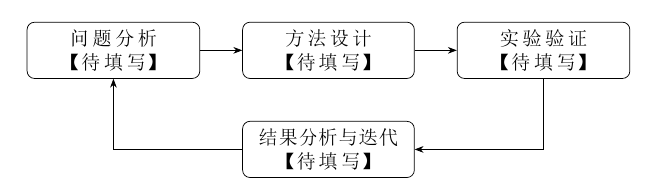
\includegraphics[width=0.8\textwidth]{pic/flowchart.png}
\caption{技术路线示例框图（请替换节点内容）}\label{fig:route}
\end{figure}

\begin{equation}
J(\theta)=\frac{1}{N}\sum_{i=1}^{N}\ell\bigl(f_{\theta}(x_i),y_i\bigr)
\label{eq:placeholder}
\end{equation}